\section{Composing Optimizations}\label{sec:composing}
After we evaluated optimizations individually, we composed the optimizations
together in hopes of aggregating the benefits of each optimization.
Unfortunately, the optimizations were not orthogonal, and composing them proved
non-trivial.

For example, loop reordering conflicted with copy optimization since the order
of the loops dictated the access patterns. Similarly, the \ttt{aligned}
annotation greatly improved the performance of the naive matrix multiplication
but had negligible effects on the optimized matrix multiplication.

For now we've prioritized the copy optimizations because they were far more
successful at increasing performance. We also had to modify where we did our
copying when combined with blocking. Since we changed one matrix to be
row-major order, we had to modify how parameters were being passed between the
functions for blocking.

The final performance of the fully optimized kernel is shown in
\figref{composed} as the line labelled \ttt{mine}.

\begin{figure}[h]
  \centering
  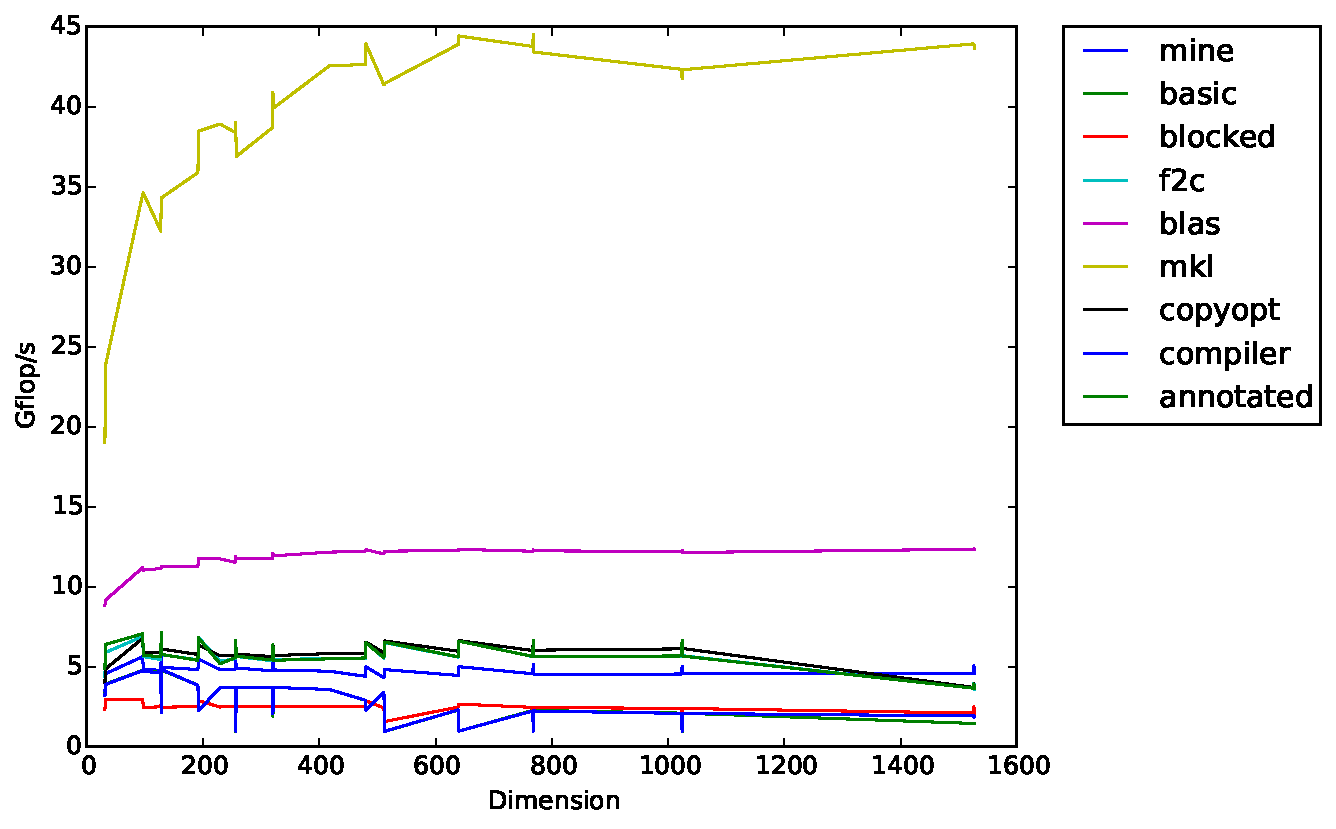
\includegraphics[width=\textwidth]{timing_composed.pdf}
  \caption{Fully optimized matrix multiplication.}
  \label{fig:composed}
\end{figure}
